\documentclass{article}
\usepackage[UTF8]{ctex}
\usepackage{geometry}
\usepackage{natbib}
\geometry{left=3.18cm,right=3.18cm,top=2.54cm,bottom=2.54cm}
\usepackage{graphicx}
\pagestyle{plain}	
\usepackage{setspace}
\usepackage{caption2}
\usepackage{datetime} %日期
\renewcommand{\today}{\number\year 年 \number\month 月 \number\day 日}
\renewcommand{\captionlabelfont}{\small}
\renewcommand{\captionfont}{\small}
\begin{document}

\begin{figure}
    \centering
    
\includegraphics[width=8cm]{upc.png}

    \label{figupc}
\end{figure}

	\begin{center}
		\quad \\
		\quad \\
		\heiti \fontsize{45}{17} \quad \quad \quad 
		\vskip 1.5cm
		\heiti \zihao{2} 《计算科学导论》课程总结报告
	\end{center}
	\vskip 2.0cm
		
	\begin{quotation}
% 	\begin{center}
		\doublespacing
		
        \zihao{4}\par\setlength\parindent{7em}
		\quad 

		学生姓名:\underline{\qquad  李坤桐 \qquad \qquad}

		学\hspace{0.61cm} 号:\underline{\qquad 1801050125\qquad}
		
		专业班级:\underline{\qquad 计科1801 \qquad  }
		
        学\hspace{0.61cm} 院:\underline{计算机科学与技术学院}
% 	\end{center}
		\vskip 2cm
		\centering
		\begin{table}[h]
            \centering 
            \zihao{4}
            \begin{tabular}{|c|c|c|c|c|c|c|}
            % 这里的rl 与表格对应可以看到,姓名是r,右对齐的;学号是l,左对齐的;若想居中,使用c关键字。
                \hline
                课程认识 & 问题思 考 & 格式规范  & IT工具  & Latex附加  & 总分 & 评阅教师 \\
                30\% & 30\% & 20\% & 20\% & 10\% &  &  \\
                \hline
                 & & & & & &\\
                & & & & & &\\
                \hline
            \end{tabular}
        \end{table}
		\vskip 2cm
		\today
	\end{quotation}

\thispagestyle{empty}
\newpage
\setcounter{page}{1}
% 在这之前是封面,在这之后是正文
\section{引言}
本课程主要包括三部分,首先是老师讲授计算学科基本知识和学科方法论,然后是同学们根据自己的兴趣选择主题并进行计算领域热点主题演讲,最后是树立目标,同学们进行个人职业规划设计。出于对“人机对弈-德州扑克”的好奇,我们小组选择了该主题进行研究。通过一学期的听课和小组研究,将我对这门课的体会和进一步思考做以下总结。

\section{对计算科学导论这门课程的认识、体会}
总的来说,在听课过程中,学会了科学哲学的思想方法,计算机科学的基本概念和基本知识,计算科学的意义、内容和方法。从宏观上对本专业有了进一步的了解。\par

\subsection{计算科学与计算机科学的区别}
我认为,计算科学更偏向于理论,而计算机科学则更偏向于技术、工程。这两个概念有很大的交叉部分,百度百科也会把它们混在一起算一个概念。如果仔细区分它们的话,也是有很多不同之处的,计算机科学(computer science,CS)是系统性研究信息与计算的理论基础以及它们在计算机系统中如何实现与应用的实用技术的学科。\citep{aa} \citep{bb}它通常被形容为对那些创造、描述以及转换信息的算法处理的系统研究。尽管计算机科学的名字里包含计算机这几个字,但实际上计算机科学相当数量的领域都不涉及计算机本身的研究。因此,一个新的名字被提出来,它就是计算科学。计算科学,又称科学计算,是一个与数学模型构建、定量分析方法以及利用计算机来分析和解决科学问题相关的研究领域。在实际应用中,计算科学主要应用于:对各个科学学科中的问题,进行计算机模拟和其他形式的计算。计算科学技术要想获得理解,主要需要通过在计算机上实现的数学模型进行分析。\par


\subsection{从李运华的文章中我学到的}
如何成为大牛?一定要找到你有激情的一份工作或者是你的事业并为之努力坚持,每天要花3小时用于提升自己的技能,这样一直做,持续大约10年时间。将一个宏大的“10年成为技术大牛”的目标,分解成1-2个月可执行的具体行动,一段分解“等级”,二段分解“技能”,为了达到一段目标,需要具备什么样的技能,三段分解“行动”,将技能目标分解为具体要做的事,然后按照计划执行。在日常学习中要做到do more、do better、do exercise。这些有效的方法也运用到了我的职业规划设计中。\par

\section{对人机对弈-德州扑克的进一步思考}
什么是德州扑克?其实它的规则对于主题的理解是十分重要的,要想机器打败人类,至少要非常清楚的知道规则,演讲时由于时间限制没有详细介绍,这里完整的说明一下德州扑克具体的玩法流程。\par
先下大小盲注,然后给每个玩家发2张底牌,大盲注后面第一个玩家选择跟注、加注或者盖牌放弃,按照顺时针方向,其他玩家依次表态,大盲注玩家最后表态,如果玩家有加注情况,前面已经跟注的玩家需要再次表态甚至多次表态。同时发三张公牌,由小盲注开始(如果小盲注已盖牌,由后面最近的玩家开始,以此类推),按照顺时针方向依次表态,玩家可以选择下注、加注、或者盖牌放弃。发第4张牌,由小盲注开始,按照顺时针方向依次表态。发第五张牌,由小盲注开始,按照顺时针方向依次表态,玩家可以选择下注、加注、或者盖牌放弃。经过前面4轮发牌和下注,剩余的玩家开始亮牌比大小,成牌最大的玩家赢取池底。比牌方法:用自己的2张底牌和5张公共牌结合在一起,选出5张牌,不论手中的牌使用几张(甚至可以不用手中的底牌),凑成最大的成牌,跟其他玩家比大小。比牌先比牌型,大的牌型大于小的牌型,牌型一般分为10种,从大到小为:同花大顺、同花顺、四条、满堂红、同花、顺子、三条、两对、一对、高牌。下注宗旨为玩家之间同时继续看牌或比牌需要下同样注额筹码,筹码不足的玩家all in全下后可以看到底并参与比牌。\par
接下来深入了解德州扑克的人机对弈程序,我们要说的是大型不完全信息游戏的人工智能,特别是关于如何在无限制扑克中击败顶级人类的人工智能。首先,我们的主题是不完全信息游戏,不会讨论象棋或围棋这样的完全信息游戏,不完全信息适用于扑克,并且更广泛地适用于任何涉及隐藏信息的战略互动,例如,安全互动或谈判。\par
我认为这对于对弈的人工智能进入现实世界非常重要,因为大多数现实世界的战略互动都涉及到一定量的隐藏信息。当谈到这些人机对弈程序时,扑克作为主要的基准挑战可以追溯到几十年前。查看一些博弈论的原始论文时,会发现他们唯一谈到的应用几乎就是扑克,因为它准确的抓住了不完全信息的挑战因素,其中特别是有一种扑克,也就是我们的主题,无限制德州扑克,已经成为检验人工智能的主要基准。\par
一个无限制的德州扑克是一个巨大的游戏,它有大约10到161个不同的决定点。它也是世界上最流行的扑克变体,是世界扑克系列赛主赛事的游戏。在关于扑克的流行电影中也有它的身影,例如,《007:大战皇家赌场》和《赌王之王》。从某种角度说,德州扑克是最纯粹的扑克形式,它是主观的,但也是一个非常有策略的游戏,完全取决于你的技术。我们很难想象AI能够在这个游戏中击败顶级人类。\par
2015年,加拿大阿尔伯塔大学Michael Bowling 等人就在《Science》上发表《Heads-up limit hold’em poker is solved》\citep{cc},首次提出可以解决单挑扑克变种(Limit Texas Hold 9em)的博弈问题,即有限制的德州扑克。这一结果是由新算法CFR +实现的,该算法能够解决比以前更大数量级的扩展形式游戏。\par
2016年,加拿大阿尔伯塔大学开发的“深筹”(DeepStack)在单挑无限注德州扑克中击败了职业扑克玩家,具有统计意义。该代码设法在一个称为对决无限制德州扑克Hold9em的两人扑克变种中击败职业扑克玩家。2017年,发表在《Science》上的文章《DeepStack: Expert-level artificial intelligence in heads-up no-limit poker》\citep{dd},介绍了深筹的对弈方法,它并没有预先设计策略,而是在考虑到游戏当前状态的每一步中对其进行了重新计算。\par
2017年1月,美国卡内基梅隆大学开发的德扑AI Libratus(冷扑大师)与 4 名人类顶尖德州扑克选手进行实战对局,这是新的突破,在20天的时间里打了12万手牌。最后的结果是,Libratus在这场比赛中战胜了顶级人类。那么这些职业选手的实力如何?因为与真正的顶级选手对战很重要,遗憾的是,职业扑克玩家没有客观的排名,但这些人都是每年在网上玩这个游戏可以赚到年薪百万的人,并且奖金池有20万美元分给职业选手,以激励他们拿出最好的状态。\par
现在我们简单说明一下为什么德扑的人机对弈游戏这么难以设计,毕竟我们已经见识过人工智能在象棋比赛、围棋比赛中击败人类。其中主要挑战之一,就是在不完全信息博弈中,一个子游戏的最优策略不能孤立地确定,即仅仅利用该子游戏的信息是无法确定的。这其实就是打败顶级人类的关键突破。 但事实证明,在扑克牌中,它的难度要大得多。在完全信息游戏中,你采取一些行动,你的对手采取一些行动,造成一个特别的子游戏,此时你可以忘掉之前的一切,忘掉其它所有没有遇到的情况,唯一重要的是你所处的情况,以及从这一点可以达到的情况。但是在不完全信息的棋局中,如果你采取了一些行动,而你的对手也采取了一些行动,你发现自己处于一个特别的子游戏中,现在其他的一些子游戏,你不在其中,甚至可能无法从这一点上达到,但却会影响到你所处的子游戏的情况。 \par
简单介绍完不完全信息博弈中子游戏的特点,我们在明确一下人机对弈程序的目标是什么。我们的目标是在两个人的零和游戏中找到一个纳什均衡,以保证不会失去一个期望值。要找到一个纳什均衡并不容易,但它在有限的两人零和游戏总是保证存在。在扑克这种复杂的游戏中,有很多次行动,实际上并没有在纳什均衡中进行,所以我们的目标是找到一个近似的纳什均衡。\par 
那么如何找到这个近似的纳什均衡,需要有一个庞大的博弈。Libratus提出了一种可行的策略,2018 年 Noam Brown 等人在《Science》发表《Superhuman AI for heads-up no-limit poker: Libratus beats top professionals》\citep{ee},详细介绍了如何用AI打德扑。我们只在博弈的早期,估计最佳策略是什么和博弈后期的预期值是什么。当我们在实际玩的时候,发现自己在一个特定的子游戏中,利用其他子游戏的期望值的信息,为这个特定的子游戏得出最佳策略。然后,重复这个过程,只是针对那个即将到来的早期部分想出最佳策略,然后我们发现自己处在那个早期的子游戏中,则再次利用其他子游戏的期望值的信息来计算特定的子游戏。这就是所谓的嵌套子游戏解法,也是找到纳什均衡和打败顶尖人类的关键突破口。\par
\begin{figure}[h!]
	\centering
	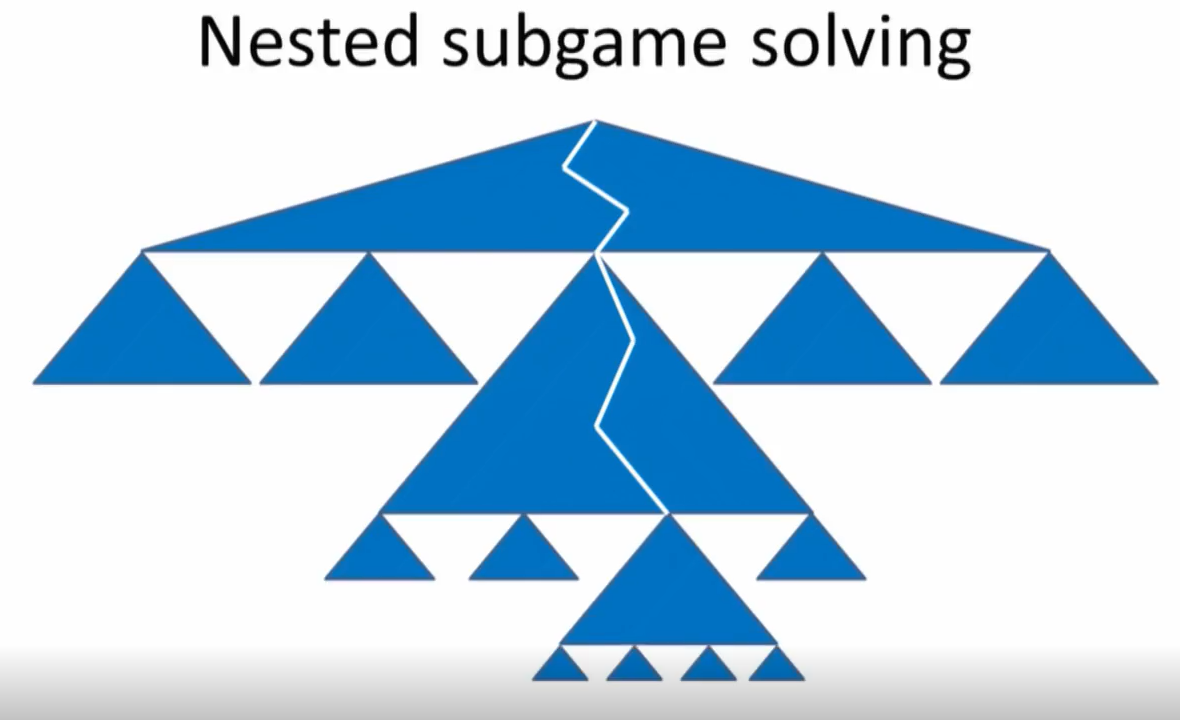
\includegraphics[scale=0.5]{a}
	\caption{嵌套子游戏}
	\label{fig:universe}
\end{figure}
在演讲中我们没有讲到AI 应对德扑多人牌局的算法,只是作为发展历程提了一下,在这里进行补充。\par
过去,所有利用AI打扑克的系统都只设置了2名玩家。所以设计一种针对多人牌局的超人类AI被普遍看做是AI发展的下一个关键节点。2019年,题为《Superhuman AI for multiplayer poker》\citep{ff}发表于《Science》,作者在这篇文章中描述了 Pluribus,一种能够在6人牌局中打败顶尖人类选手的新型AI系统。这个系统是18年提出的Libratus的改进升级版,下面主要是对这篇论文进行简要分析。\par
由于模型特性和纳什均衡性质,我们可以证明:在双人零和博弈模型中,倘若应用纳什均衡策略则至少可以保证不输,之前那些AI算法取得成功的原因:不遗余力寻找纳什均衡。但是面对更复杂的问题,纳什均衡就心有余而力不足了。目前还没有一种能在多项式时间内找到双人非零和博弈纳什均衡的算法。就算是零和博弈,想找到3人或更多玩家零和博弈的纳什均衡也是十分困难的。
即使在多人博弈中每个玩家都得到了纳什均衡策略,这样执行下来的结果未必是纳什均衡的,Lemonade stand game就是一个典型例子\citep{gg}。在 Lemonade stand game 中多个玩家同时在一个圆环上选择位置,目标是距离别人越远越好。这个博弈的纳什均衡是每个玩家在圆环上均匀分布,能达到这样效果的策略有无数多种,倘若每个玩家独立计算一种,则产生的联合策略不一定是纳什均衡,如图所示。\par
\begin{figure}[h!]
	\centering
	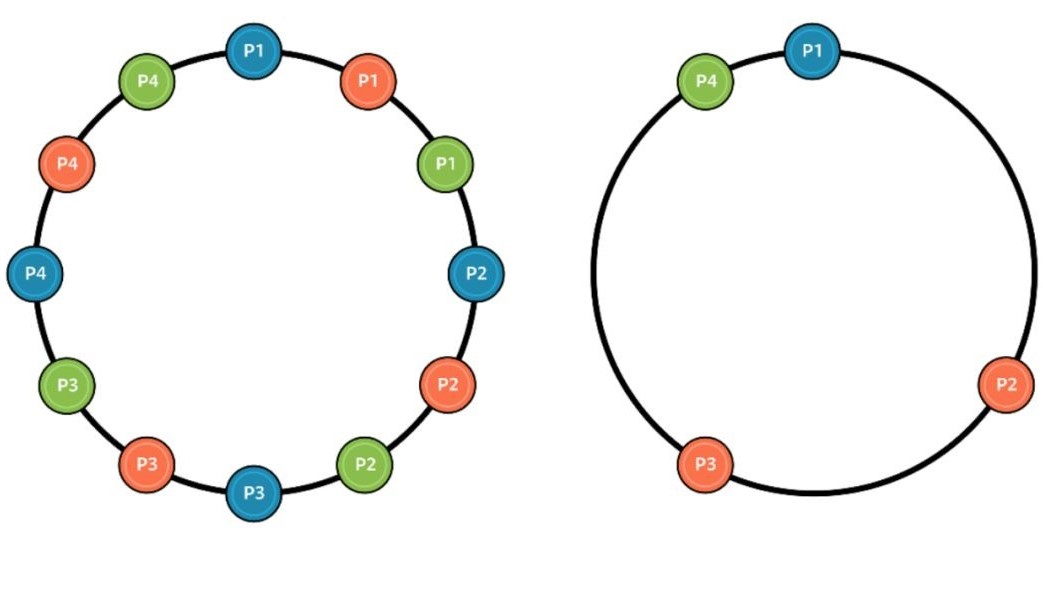
\includegraphics[scale=0.5]{b}
	\caption{Lemonade stand game}
	\label{fig:universe}
\end{figure}
纳什均衡的短板引发了众多科学家的思考:面对此类博弈问题,我们该如何解决。因此,作者认为在6人牌局中,我们的目标不应该是去寻找某一种特定的博弈理论求解,而是创建一个能够以经验为主的可以持续击败人类的AI系统。作者提出了Pluribus程序,尽管在理论上作者无法保证最后的策略一定是纳什均衡的,但是通过观察实验发现,所设计的AI系统能够稳定地以某种强策略击败顶级人类玩家。虽然这样的技术没有足够的理论支撑,但是仍然都够在更为广阔的领域产生更多超人策略。\par
Pluribus策略核心是持续不断地进行自学习自博弈,也就是说在这样的训练方式中,AI系统只和自己的镜像进行对抗,而不获取任何人类游戏数据或先前的AI游戏数据。起初,AI随机选择玩法,然后逐步改变其行动并确定行动的概率分布,最终,AI的表现会取得明显提升。作者称Pluribus利用自学习制定的离线策略为“蓝图策略”,随着真实游戏的进行,Pluribus通过在比赛中自己的实际情况实时搜索更好的策略来改进蓝图策略。\par
无限制的德州扑克中有太多的决策点可以单独推理。为了降低游戏的复杂性,作者消除了一些考虑因素并且将类似的决策点放在一起,这个过程称之为抽象。在抽象之后,划分的决策点被视为相同决策。作者在Pluribus中使用了两种抽象:动作抽象和信息抽象。\par
动作抽象减少了AI所需要考虑的动作数。在无限制的德扑中,通常允许玩家在100刀至10000刀之间进行任意价格投注。但是,在现实情况中投注200刀和201刀几乎没有区别。为了降低形成策略的复杂性,Pluribus在任何给定的决策点只考虑几种不同的下注大小。它所考虑的确切投注数量在1到14之间变化,具体取决于具体情况。\par
信息抽象对于所揭示信息(如玩家的牌和显示的牌)类似的决策点进行合并。举例来说 10-high str AI ght 和 9-high str AI ght 在牌型上差距明显,但是策略层面却是相似的。Pluribus可以将这些牌型放在一起并对其进行相同的处理,从而减少了确定策略所需的不同情况的数量。信息抽象大大降低了游戏的复杂性,但它可能会消除一些对于超人表现来说非常重要的微妙差异。因此,在与人类的实际比赛中,Pluribus 仅使用信息抽象来推断未来下注轮次的情况,而不是实际所在的下注轮次。\par
Pluribus所使用的蓝图策略是CFR中的一种。CFR是一种迭自学习训练算法,AI从完全随机开始,通过学习击败其早期版本逐渐改进。过去6年间几乎所有德扑AI都采用了CFR变形中的一种。在本文中,作者采用一种蒙特卡洛CFR(Monte Carlo CFR)方法对博弈树上的行动进行采样而不是在每次迭代时遍历博弈树。\par
在每次算法迭代中,MCCFR指定一名玩家为遍历者,他的当前策略将在迭代时更新。迭代开始时,MCCFR会根据所有玩家的当前策略模拟一手牌。一旦模拟结束,AI就会审查遍历者做出的每个决定,并考虑如果采用其他可行行动会更好还是更差。接下来,AI会考虑在其他可行行动之后可能做出的每个假设决策,考虑其行动更好还是更差,以此往复。博弈树如图所示。\par
\begin{figure}[h!]
	\centering
	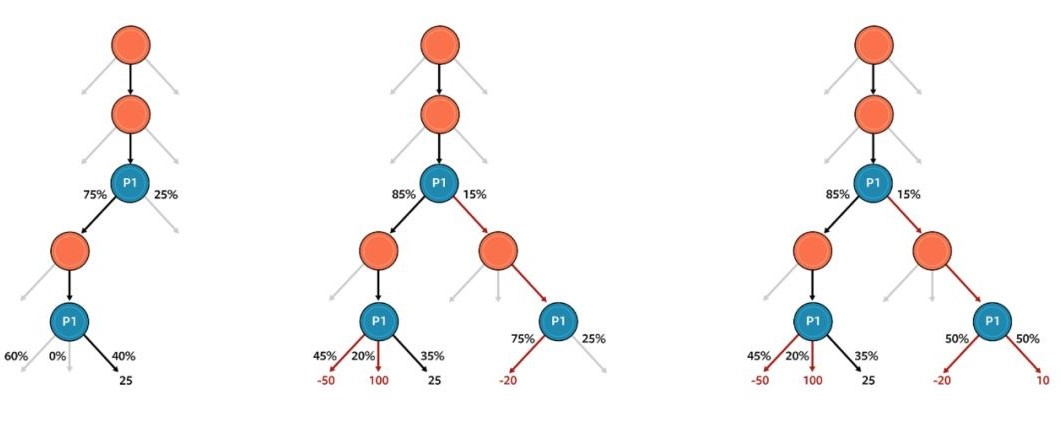
\includegraphics[scale=0.6]{c}
	\caption{博弈树}
	\label{fig:universe}
\end{figure}
由于无限制德州扑克的规模和复杂性,整个游戏的蓝图策略必然是粗粒度的。Pluribus 仅仅在第一轮下注时根据蓝图策略进行游戏,其中决策点的数量足够小,以至于蓝图策略可以承受不使用信息抽象并且在动作抽象中选择更多动作。 在第一轮之后(即使在第一轮中,如果对手选择的赌注大小与蓝图动作抽象中的大小完全不同),Pluribus也会进行实时搜索,以确定更好,更细粒度的策略。对于在第一轮稍稍偏离博弈树的对手投注,Pluribus 使用 pseudoharmonic mapping将赌注映射到附近的on tree赌注上并继续根据蓝图进行游戏,就好像对手真的使用了这样的赌注大小。\par
在许多完全信息博弈中实时搜索对于实现超人类表现是非常重要和必要的。这种情况下国际AI通常会向前看一些移动,直到在算法前瞻的深度限制处到达叶节点。原则上,如果 AI可以准确地计算每个叶节点的值(例如取胜,平局或失败),则该算法将选择最佳的下一步动作。但是这样的搜索方法在不完全信息博弈中完全不适合。\par
Pluribus使用一种新方法,其中搜索者明确地认为任何或所有玩家可以转移到子博弈的叶节点之外的不同策略。作者假设当到达叶子节点时,每个玩家可以在k个不同的策略之间进行选择以进行接下来的博弈。在本文中作者设定k=4。第一种是预先计算的蓝图策略;第二种是一种改进的倾向于folding的蓝图策略;第三种是倾向于calling的蓝图策略;第四种是倾向于raising的蓝图策略。(以上folding、calling、raising均为牌桌策略,分别为弃牌、跟注和加注)\par
这种技术的引进将使得探索者找到更平衡的策略,因为选择不平衡策略(例如总是出石头)将被对手转移到其他策略(例如总是出布)惩罚。\par
在不完全信息博弈中搜索的另一个主要挑战是,玩家在特定情况下的最佳策略取决于从对手的角度看,玩家在每个情况下的策略是什么。为了应对这一挑战,Pluribus 根据其策略跟踪每副手牌可能达到当前状况的概率。\par 无论Pluribus实际持有哪手牌,它都会先计算出每一手牌的动作方式,小心平衡所有牌局的策略,以保持不可预测性。一旦计算出所有人的平衡策略,Pluribus就会为它实际持有的牌执行一个动作。 在Pluribus中使用的深度限制的不完全信息子博弈的结构如图所示。\par
\begin{figure}[h!]
	\centering
	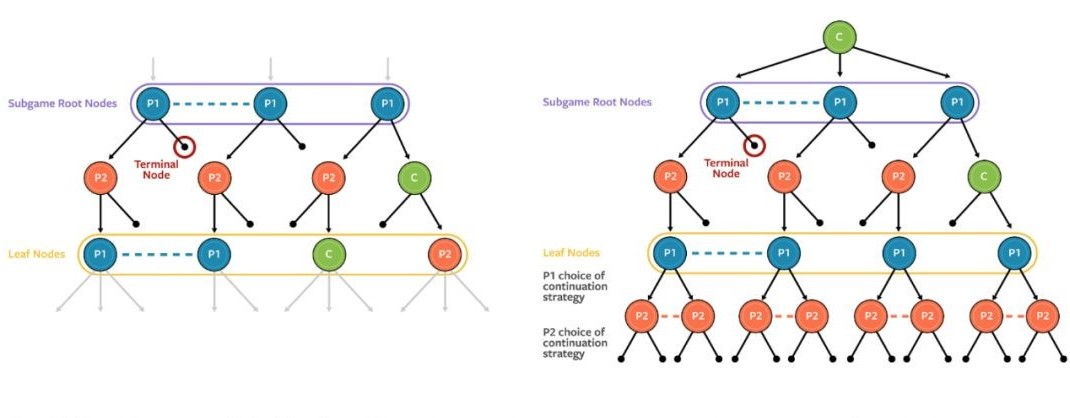
\includegraphics[scale=0.6]{d}
	\caption{不完全信息子博弈}
	\label{fig:universe}
\end{figure}
Pluribus使用两种不同形式的 CFR 来计算子博弈中的策略,具体取决于子博弈的大小和游戏进行的位置。如果子博弈相对较大或者在游戏的早期,则使用和蓝图策略一样的蒙特卡罗线性CFR。否则,Pluribus使用优化的基于矢量的线性CFR形式仅对机会事件(例如公共牌)进行采样。\par
实际测试时,Pluribus仅仅使用了两台 Intel Haswell E5-2695 v3 CPU,仅占用小于128G 的内存。相比而言,AlphaGo 对阵李世石时使用了1920块CPU和280块GPU。在对每一个子博弈进行搜索时,根据现场情况,Pluribus仅需要 1-33 秒。在其与自己镜像对抗的 6 人牌局中平均出牌时间为20s,这远比顶尖人类选手快了近乎2倍。\par
Pluribus 这次出彩的表现使得AI多人游戏不再是难以逾越的鸿沟。也说明面对更复杂的情况和场景,即使难以取得理论支撑,倘若合理建模、合理设计算法,则从实践上先行突破也未必不可行。此外,人们潜意识中,训练=资源=烧显卡。此次Pluribus的成功无疑使得众多“科研平民”看到了希望和曙光。Pluribus成功应用于德扑也增强了科研工作者将 AI 推广于更复杂更广泛领域的信心。\par
演讲中有提到人机对弈的拓展应用,有消息透露冷扑大师正在为美国军方进行秘密研究,演讲结束后老师提到人机对弈技术研究的初衷就是为了应用于军事,这是我之前没有关注过的点,所以后续又查找了一些资料进行了解和学习。\par
随着深度学习、强化学习等新一代人工智能技术的发展, 其在计算机视觉、语音识别、自然语言处理、生物医疗领域及游戏博弈等方面取得很大的突破, 人工智能在军事领域应用也愈加广泛, 催生了军事智能的概念\citep{hh}。其中一个重要概念就是人机混合智能,人机混合智能中又有一部分是关于博弈智能化的。\par
早在20 世纪50 年代末,美国军方的共识是,其指挥与控制系统不能满足日益复杂和快速多变的军事环境下快速决策的紧迫需求,1961 年肯尼迪总统要求军队改善指挥与控制系统。在该国防安全重大问题提出以后,国防部指派DARPA负责此项目。为此DARPA成立了信息处理技术办公室,并邀请麻省理工学院约瑟夫•利克莱德教授出任首任主任。虽然是军方的迫切需要和总统钦定的问题,但DARPA没有陷入军种的眼前需求和具体问题,而是基于利克莱德提出“人机共生”的思想,认为人机交互是指挥与控制问题本质,并就此开展长期、持续的研究工作。此后,IPTO遵循着利克莱德的思想逐渐开辟出计算机科学与信息处理技术方面的很多新领域,培育出ArpaNet等划时代颠覆性技术,产生了深远的影响,直至今天。\par
从战争需求的视角看,博弈智能化会对军事变革有一定的影响趋势,包括催生更多的“聪明”武器和自主化无人平台、使指挥员对战场态势的认知速度大幅提高、使指挥信息系统克服智能辅助上的瓶颈、助推兵棋推演实现真正的人机对抗、拓展认识信息化战争机理的新途径等等,都有可能实现。\par



\section{总结}
通过本课程,我受益良多,不仅学习了很多新知识,开阔了视野,同时坚定了我努力学习专业知识的决心。了解了学科重要的基本概念和学科方法论,学会了常见的信息检索方法,学会了使用一个文档编辑软件-latex,了解了IT领域目前的最新趋势、研究热点和前沿知识。对未来有了更清晰的认识,做出了比较详细的职业规划设计,充分认识到终身学习的重要性,树立了较强的自主学习和终身学习意识。感谢老师的悉心指导,我一定会不断努力。\par


\section{附录}
\begin{itemize}
    \item Github个人网址:https://github.com/wenny-kiki
    \item CSDN个人网址:https://blog.csdn.net/weixin\_46090517
    \item 博客园个人网址:https://www.cnblogs.com/-TheMilkyWay/
    \item 小木虫个人网址:http://muchong.com/bbs/space.php?uid=21967053

\begin{figure}[h!]
	\centering
	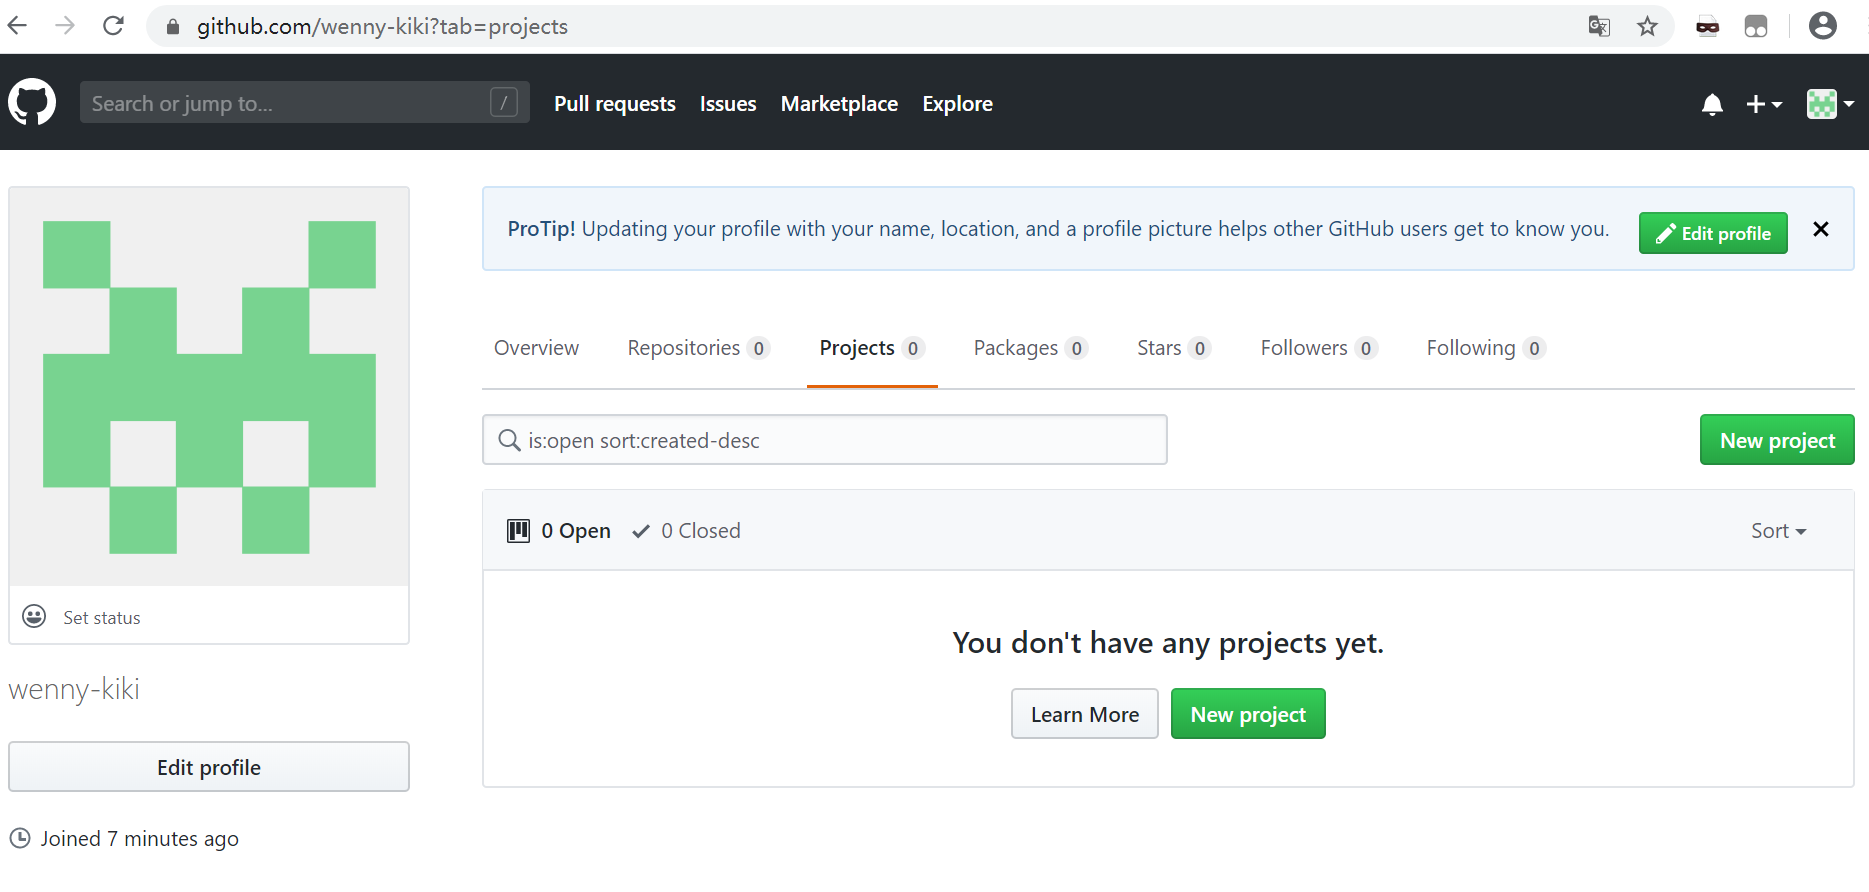
\includegraphics[scale=0.45]{github}
	\caption{Github截图}
	\label{fig:universe}
\end{figure}
\begin{figure}[h!]
	\centering
	
\includegraphics[scale=0.46]{csdn}
	\caption{CSDN截图}
	\label{fig:csdn}
\end{figure}
\begin{figure}[h!]
	\centering
	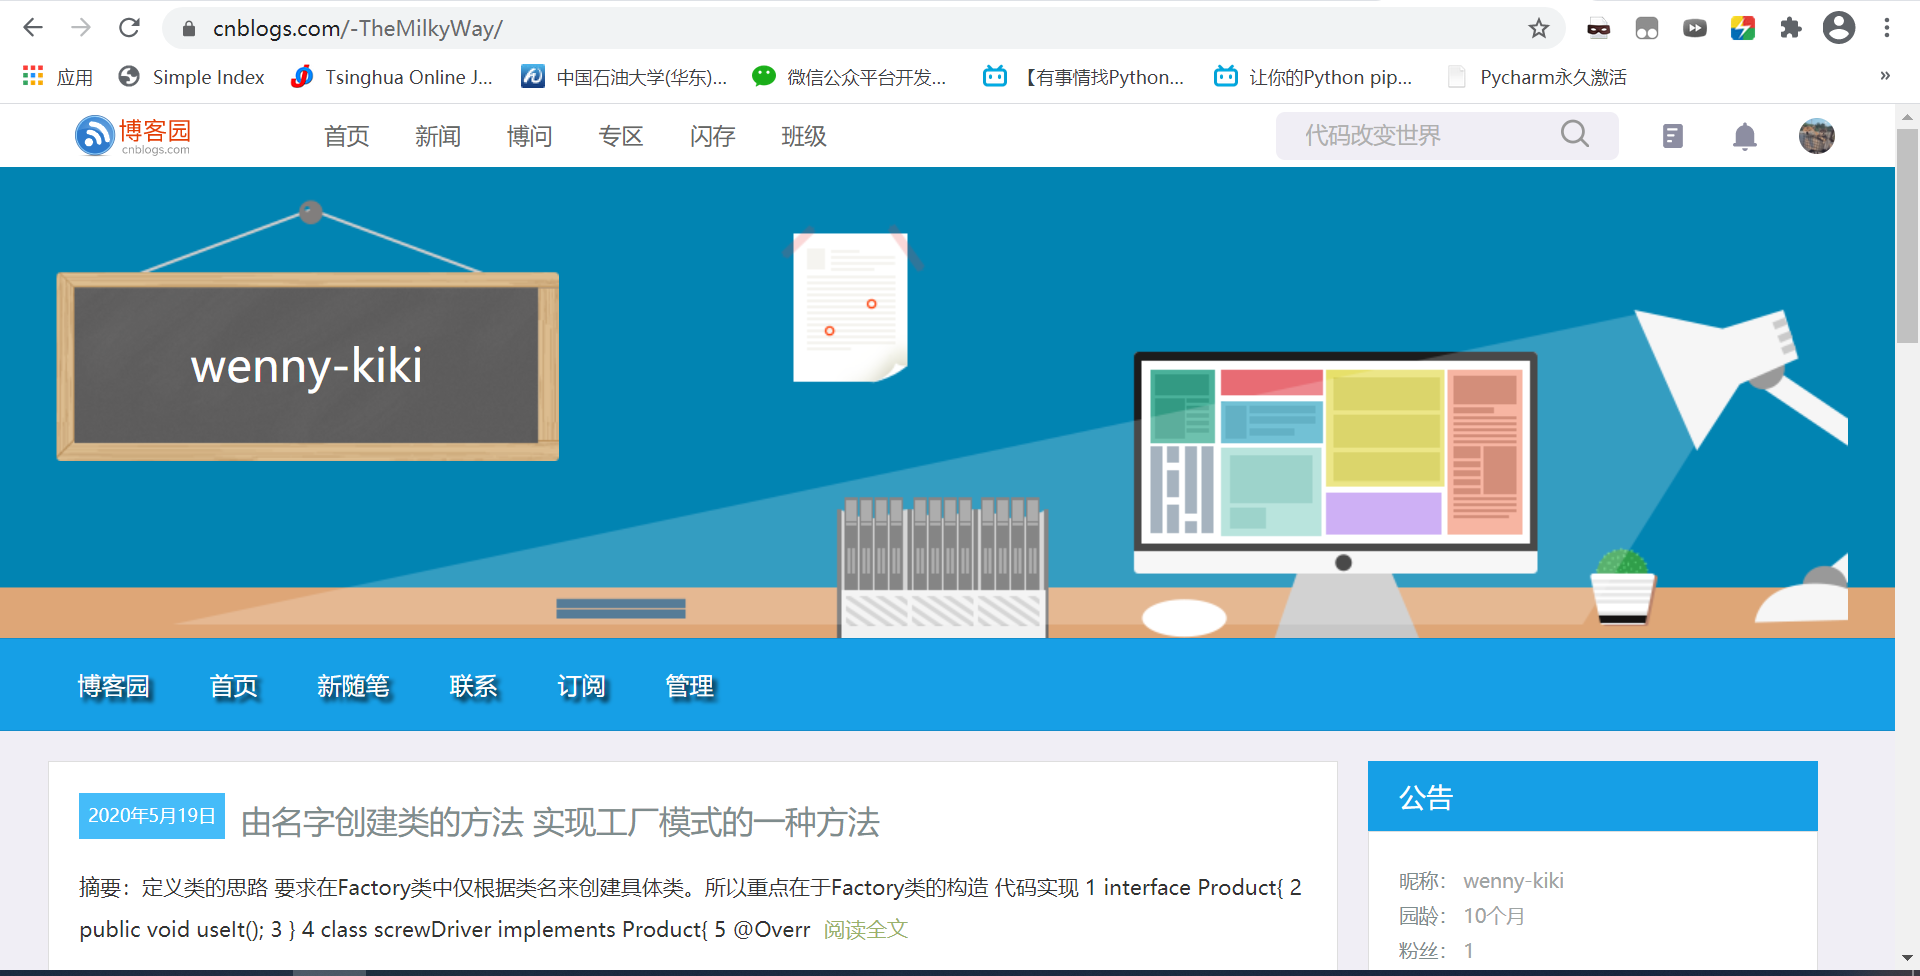
\includegraphics[scale=0.5]{bokeyuan}
	\caption{博客园截图}
	\label{fig:universe}
\end{figure}
\begin{figure}[h!]
\centering

\includegraphics[scale=0.15]{xuexi}
\caption{学习强国截图}
\label{fig:universe}
\end{figure}
\begin{figure}[h!]
	\centering
	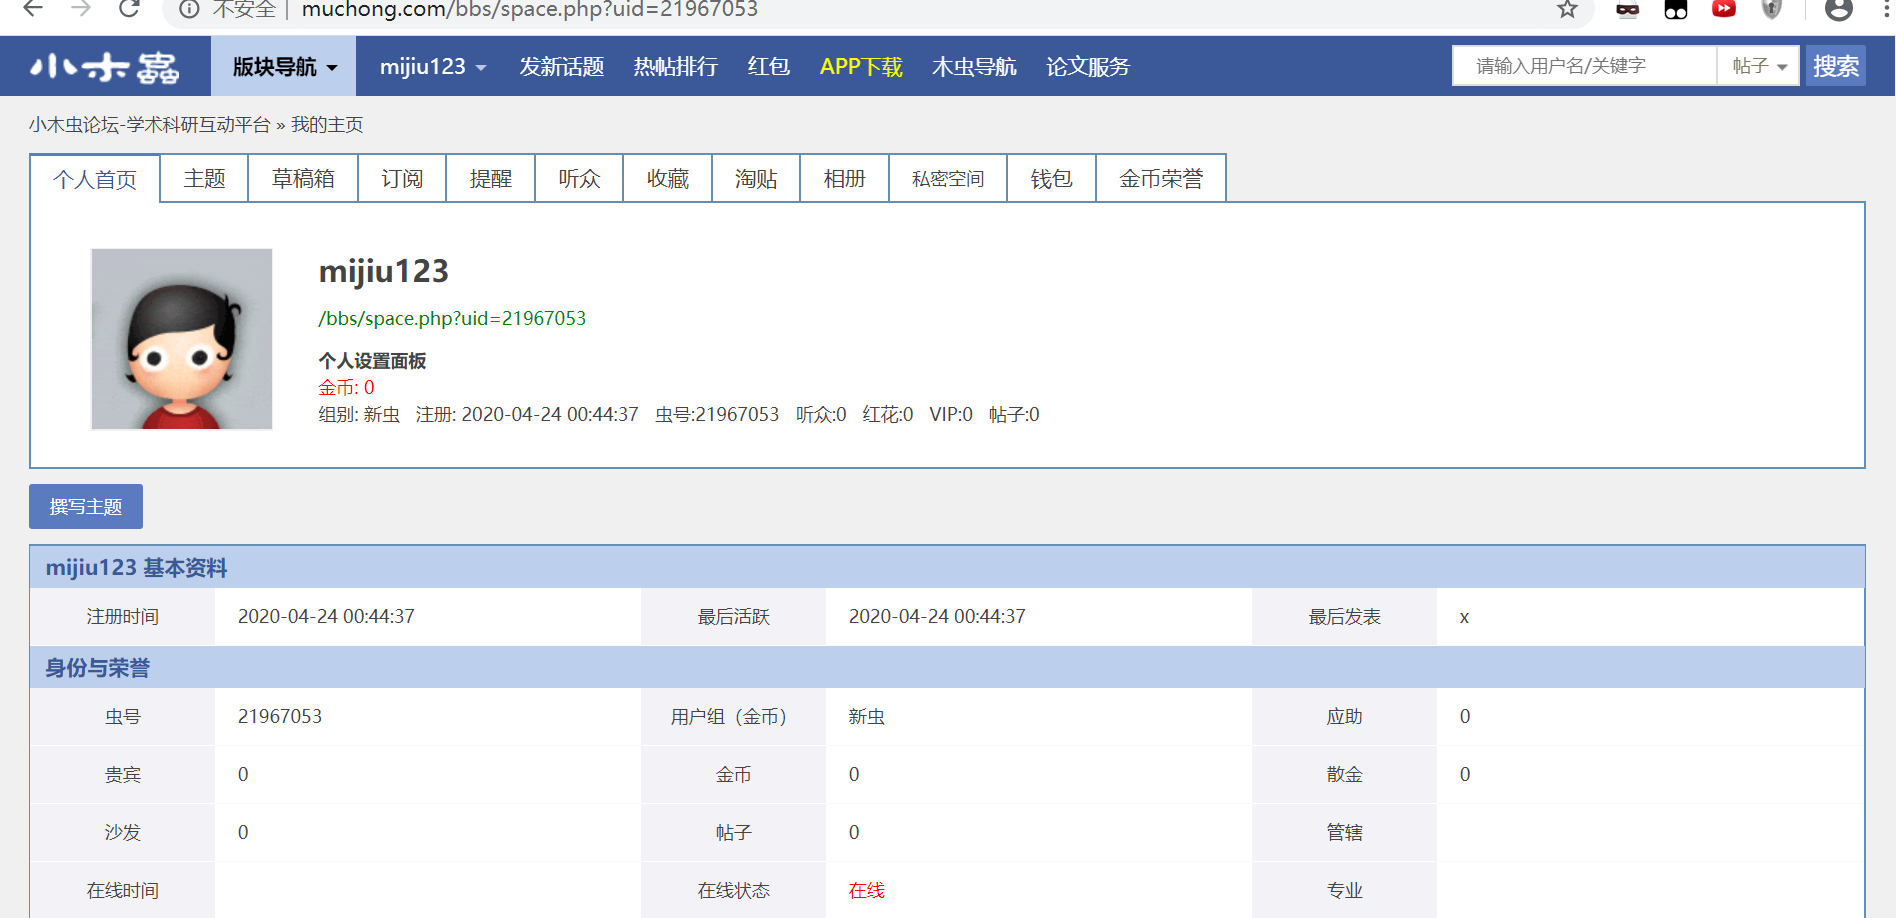
\includegraphics[scale=0.4]{xiaomuchong}
	\caption{小木虫截图}
	\label{fig:universe}
\end{figure}


\begin{figure}[h!]
	\centering
	
\includegraphics[scale=0.4]{bilibili}
	\caption{bilibili截图}
	\label{fig:universe}
\end{figure}
\end{itemize}

\hspace*{\fill} \\
\bibliographystyle{plain}
\bibliography{references}


\end{document}
